% !TeX spellcheck = en_GB
% !TEX root = ../thesis.tex


\chapter{Solutions with broken time-translation symmetry} \label{ch:hopf}


\begin{chapterabstract}
	
	
The time-dependent systems presented so far in this thesis were subject to some periodic external drive, which allowed us to use the method of harmonic balance. Here, we explore the physical consequences of this periodicity -- or discrete time-translation symmetry (DTTS) -- of the problem. We shall see that, depending on the harmonics present in our system's behaviour, imposing DTTS implies a degeneracy of steady state solutions. This degeneracy may be discrete, corresponding to the generation of subharmonics. It may also be continuous, which gives rise to a $U(1)$ gauge freedom of the system, resulting in aperiodic solutions known as limit cycles. Due to the infinite degeneracy implied by the gauge freedom, limit cycles cannot be captured by the standard harmonic balance method. We develop an approach for fixing this gauge, which allows us to numerically characterise limit cycle behaviour. Finally, we consider adiabatic transitions within the continuous solution space and thus arrive at the notion of a geometric phase.
%
\tcblower
%
The methods developed here have been incorporated into HarmonicBalance.jl~\cite{Kosata_2022a}, which was used to produce the presented data. For more details, see the documentation~\cite{harmonic_balance_docs}.
\end{chapterabstract}

Although not explicitly stated, all time-dependent systems presented so far in this thesis have possessed DTTS. In terms of our general equation of motion \eqref{eq:hb_general_ode}, this means, for DTTS with period $\tau$,
\begin{equation} \label{eq:hopf_dtts}
\vb{G}(\vb{x}(t), t)=\vb{G}(\vb{x}(t), t+\tau)=\vb{G}(\vb{x}(t-\tau), t)=0\:.
\end{equation}
Equivalently, one may impose $H(t + \tau) = H(t)$ for the underlying time-dependent Hamiltonian $H(t)$. The period $\tau$ typically results from the presence of a periodic drive at frequency $\omega = 2\pi / \tau$. The second equality in Eq.~\eqref{eq:hopf_dtts} implies that for each solution $x(t)$, we may generate another one, $x(t-\tau)$. In this Chapter, we explore the implications of this symmetry. 

It is important to contrast the DTTS presented here to spatial translation symmetry, which played a key role in Part \ref{part:spatial}. Recall that this allowed us to use the powerful results of representation theory, under the condition that the system is linear. For our nonlinear time-dependent systems, the use of symmetry is somewhat limited, as the tabulated group representations used in Chapter~\ref{ch:symmetry} do not apply. Nevertheless, nonlinearity does not invalidate the principle of DTTS. 

\section{Symmetry-broken steady states}

For the purpose of this introduction, we are going to use the complex form of the harmonic ansatz, as introduced in Eq.~\eqref{eq:hb_ansatz_a}. Assuming for simplicity a system described by a single variable $x(t)$, we use the vector notation
\begin{equation} \label{eq:hopf_ansatz_gen}
	x(t) = \sum_{k=1}^M a_{k}(T) \e^{i \omega_{k} t } + \text{c.c}  \equiv  \sum_{k=1}^M  \left[\e^{i \tilde{\omega} t} \vb{a}(T)  + \text{c.c.}\right]_k \,,
\end{equation}
where $\tilde{\omega} =  \text{diag}(\omega_1, \ldots, \omega_M)$ is a matrix of the chosen harmonics and
\begin{equation} \label{eq:hopf_a}
\vb{a}(T) = \mqty(a_1(T) \\ \vdots \\ a_M(T))
\end{equation}
contains the harmonic variables. Within this ansatz, the time-translation operator $\mathcal{T}$ takes the form of a diagonal matrix multiplying each of the harmonic variables by a phase,
\begin{equation}
\mathcal{T}(\tau) = \text{diag}(\e^{i \omega_1 \tau} , \,, \e^{ i \omega_2 \tau} \,, \ldots \e^{i \omega_M \tau}) \,. 
\end{equation}
The action of $\mathcal{T}(\tau)$ on a solution $\vb{a}(T)$ is therefore determined by which harmonics are chosen for the ansatz \eqref{eq:hopf_ansatz_gen}. As mentioned in Sec.~\ref{sec:hb}, this choice is to some extent arbitrary and we often use different harmonics for different layers of approximation of the same problem. Here we will not dwell on this issue, merely assume that an appropriate set of harmonics has been chosen. 

Let us now consider a system whose equations of motion possess DTTS corresponding to a period $\tau$, or equivalently a frequency $\omega = 2\pi / \tau$. Often, using an ansatz with a single harmonic, $\omega$, is entirely sufficient to capture the behaviour such a system -- this was indeed the case for our single-mode model in Sec.~\ref{sec:hb}. The discrete time-translation (DTT) operator then becomes a unit matrix, $\mathcal{T}(\tau) = \mathbb{1}$. This also holds if integer multiples of $\omega$ are used for the harmonic expansion, such as in the two-mode model in Sec.~\ref{sec:hb}. 

The situation changes if other harmonics than $\omega$ and its multiples are present. Depending on the ratio of $\omega$ and the newly-emergent harmonics, we may distinguish between two scenarios. 

\subsection{Discrete case -- subharmonics} \label{sec:hopf_discrete}
When all harmonics $\omega_j$ constituting $x(t)$ are such that the ratio $\omega_j / \omega$ is a rational number, but not an integer for at least one $\omega_j$, we speak of \textit{subharmonic generation}. The oscillator then responds (partially, at least) at a fraction of the drive frequency. Denoting $\omega_j / \omega \equiv p / q$, the DTT operator $\mathcal{T}(\tau)$ then satisfies
\begin{equation} \label{eq:hopf_DTT}
\mathcal{T}(\tau)^q = \mathbb{1} \, .
\end{equation}
This has profound implications on the degeneracy of the solutions\footnote{Although we focus on steady states here, the arguments are also valid for transient solutions.}, as each $\vb{a}(T)$ can be mapped into $q$ degenerate solutions by the action of $\mathcal{T}(\tau)$. In the language of group theory, the group of DTT operations is isomorphic to a $q$-th order finite subgroup of the Lie group $U(1)$. More specifically, the DTT operations can be mapped to a set of unit complex numbers with arguments $0, \, 2\pi/q,\,, \ldots 2\pi(q-1)/q$. Correspondingly, applying a DTT operation to a steady-state solution changes the phases of its constituent harmonics.

A prominent example of this phenomenon is the parametric oscillator -- an oscillator whose natural frequency is varied periodically in time~\cite{Rand_2005, Papariello_2016},
\begin{equation}
\ddot{x}(t) + \gamma \dot {x}(t) + \omega_0^2 \left[1 + \lambda \cos(\omega t)\right] x(t) = 0\,.
\end{equation}
Beyond the critical threshold $\lambda_{\rm th} = 2 \gamma / \omega_0$, two steady states oscillating at $\omega/2$ appear (i.e., $p/q = 1/2$), distinguished from each other by phase $\pi$. Another known example is the driven Duffing oscillator,
\begin{equation} \label{eq:hopf_duffing}
\ddot{x}(t) + \gamma \dot{x}(t) + \omega_0^2 x(t) + \alpha x(t)^3 = F \cos(\omega t + \psi) \,,
\end{equation}
which, when driven at $\omega \cong 3 \omega_0$, displays a response at frequency $\omega/3$, that is, $p/q=1/3$~\cite{Arndt_2022, Jordan_Smith}. In both of these systems, the appearance of subharmonics can be seen as an instability with respect to the formation of new harmonics that resonantly interact with the drive via the nonlinear and/or parametric terms\footnote{Such instabilities are often analysed using the \textit{Hill determinant}~\cite{Richards}.}. For example, in the $p/q = 1/3$ case, the cubic nonlinearity facilitates the conversion of motion at $\omega$ and $\omega/3$ into motion at $\omega/3$ -- this is known as \textit{internal resonance}~\cite{Nayfeh_Mook, Manevich}. Intuitively, the subharmonic $\omega/3$ tends to appear where this is close to the natural frequency $\omega_0$. 

To exemplify the solution degeneracy and to further demonstrate the strength of harmonic balance combined with homotopy continuation, we attempt a variation of the Duffing subharmonic problem. Based on our internal resonance argument, we conjecture a similar process when driving at $\omega \cong 5 \omega_0$, with harmonics $\omega,\, 3\omega/5$ and $\omega /5$ constituting in the response. This necessitates a 6-variable harmonic ansatz (we drop the $T$ dependence for brevity)
\begin{multline} \label{eq:hopf_5_ansatz}
x(t) = u_1 \cos(\omega t / 5) + v_1 \sin(\omega t / 5) \\
+ u_2 \cos(3\omega t / 5) + v_2 \sin(3\omega t / 5) +  u_3 \cos(\omega t) + v_3 \sin(\omega t) \,,
\end{multline}
which gives rise to 6 coupled harmonic equations (see Appendix~\ref{app:duff_subharm}). Steady states are hence obtained by solving 6 coupled cubic polynomials. 

\begin{figure}[h!]
	\centering
	\includesvg{figures/limit_cycles/duff_sub_atan.svg}
	\caption{Stable (full, dashed) and unstable (dotted) steady states of the Duffing resonator driven near 5 times its resonant frequency $\omega_0$. Amplitudes of the harmonics (a) $\omega/5$, (b) $3\omega /5$ and (c) $\omega$ are shown. Orange branches are five-fold degenerate in amplitude. Parameters used: $\omega_0 = 1 \,, \alpha = 1 \,, F = 0.5 \,, \gamma = 10^{-4}, \psi=0$. The code used to generate this data is shown in Appendix \ref{sec:app_duffing_example}.}
	\label{fig:hb_duff_sub}
\end{figure}

The results (see Fig.~\ref{fig:hb_duff_sub}) show three different kinds of steady states. First, there is an inactive branch (blue) where all three harmonics are negligible. Second, there is a branch (red) which shows a high amplitude at $\omega$ (variables $u_3, v_3$) but zero amplitudes at $\omega/5$ and $\omega/3$. 
Third, DTTS-broken branches (orange) appear above $\omega=1.05$. Here, the response is dominated by $\omega/5$ (variables $u_1, v_1$).  
In line with our interpretation of Eq.~\eqref{eq:hopf_DTT}, we see in Fig.~\ref{fig:hb_duff_sub}(d) these branches are five-fold degenerate -- there are 5 distinct phases the response can assume with respect to the drive.

In the DTTS-broken branches, responses at $\omega/3$ and $\omega$, while very small, play a crucial role in mediating the frequency conversion. If either of the three harmonics is dropped from the ansatz, these branches never appear. 

Before leaving this topic, we stress that subharmonic generation cannot be captured perturbatively. While in cases like high-harmonic generation, new emergent harmonics may be treated as perturbations of a pre-existing steady state, subharmonics typically result from an instability and may very well dominate the response, as we have seen in our example. A similar situation occurs in the parametric oscillator. 

\subsection{Continuous case -- incommensurate harmonics} 

An altogether different situation arises when the ratio $\omega_j / \omega$ becomes irrational for at least one $\omega_j$. This means a frequency incommensurate with $\omega$ has emerged in the system's response, rendering the DTT operations isomorphic to $U(1)$ instead of its finite subgroup. Correspondingly, the solution degeneracy implied by our preceding discussion is no longer discrete, but continuous -- repeated actions of $\mathcal{T}(\tau)$ now generate an infinite set of phase-shifted solutions. 

Unlike in the DTTS-breaking case, finding the resulting steady states is not straightforward due to the seemingly arbitrary origins of an incommensurate frequency appearing in the system -- it is not clear what harmonic to add to our ansatz. Existing works overwhelmingly reach for a time-dependent simulation to find one solution at a time. We adapt the harmonic balance framework to calculate the emergent frequencies in Sec.~\ref{sec:hopf_hb}. Before proceeding however, we must delve deeper into the origins of this phenomenon. 

\subsubsection{Limit cycles from a Hopf bifurcation}

In Chapters \ref{ch:hb} and \ref{ch:linresp}, we dealt with the harmonic equations, i.e., first-order ODEs for the harmonic variables $\vb{U}(T)$,
\begin{equation}
\frac{d\vb{U}(T)}{dT}  = \bar{\vb{G}} (\vb{U})\,.
\end{equation}
These equations have no explicit time-dependence -- they are \textit{autonomous}. We have mostly been searching for steady states, which likewise show no time dependence. However, time-dependent solutions to autonomous ODEs can also exist. One mechanism for their creation is a \textit{Hopf bifurcation}~\cite{Jordan_Smith, Strogatz} -- a critical point where a stable solution transitions into an unstable one. For a stable solution, the associated eigenvalues $\lambda$ of the linearisation [see Eq.~\eqref{eq:linresp_eom}] all satisfy $\re{\lambda} < 0$. When a Hopf bifurcation takes place, one complex-conjugate pair of eigenvalues\footnote{By construction of Eq.~\eqref{eq:linresp_eom}, the eigenvalues of $J^{-1} J_0$ occur in complex conjugate pairs, since all the $J$ matrices are real.} crosses the real axis such that $\re{\lambda} > 0$. The state is then, strictly speaking, unstable. However, instead of evolving into another steady state, the system may assume a periodic orbit in phase space, giving a solution of the form 
\begin{equation} \label{eq:hopf_hopf}
\vb{U}(T) = \vb{U}_0 + \vb{U}_{\rm lc} \cos(\omega_{\rm lc} T + \phi ) \,,
\end{equation}
which is an example of a \textit{limit cycle}. We denote the originating steady state as \textit{Hopf-unstable}. 

We can continue to use harmonic balance as Eq.~\eqref{eq:hopf_hopf} still describes a harmonic response~\cite{Allwright_1977}. We will, however, first translate back to the the lab frame [variable $x(t)$], analogously to how we obtained Eq.~\eqref{eq:recons} in our treatment of linear response. Clearly, for each frequency $\omega_j$ constituting our harmonic ansatz [see Eq.~\eqref{eq:hb_ansatz}], we obtain frequencies $\omega_j$ as well as $\omega_j \pm \omega_{\rm lc}$ in the lab frame. 
Furthermore, as multiple harmonics now co-exist in the system, frequency conversion (see Sec.~\ref{sec:harm_exp}) may take place, spawning further pairs $\omega_j \pm k \omega_{\rm lc} $ with integer $k$. Therefore, to construct a harmonic ansatz capturing limit cycles, we simply add an integer number $K$ of such pairs to our existing set of $M$ harmonics,
\begin{equation}
\{ \omega_1, \ldots\,, \omega_M \} \rightarrow \{\omega_1, \omega_1 \pm \omega_{\rm lc} \,, \omega_1 \pm 2 \omega_{\rm lc}\,, \ldots\,, \omega_M \pm K \omega_{\rm lc} \} \,.
\end{equation}
Note that this implies an aperiodic response, which is analogous to the lack of translation symmetry in a quasicrystal~\cite{Pizzi_2019, Giergiel_2019}. The limit of large $K$ describes the so-called \textit{frequency combs}, which are a subject of intense research in nonlinear optics~\cite{Weng_2022, Lugiato_2018, Herr_2012}, but also appear in mechanical~\cite{Ochs_2022, Dykman2019, Czaplewski_2019, Ganesan_2018, Ganesan2017} and polaritonic systems~\cite{Zambon_2020}.

\section{Limit cycles via harmonic balance} \label{sec:hopf_hb}

Having seen how limit cycles are formed, we now proceed to tackle a key problem: how to find their frequency $\omega_{\rm lc}$. We again demonstrate by considering a single variable $x(t)$.

\subsubsection{Original ansatz}

We may try the simplest ansatz for a system driven at frequency $\omega$,
\begin{equation} \label{eq:hopf_simple_ansatz}
 x(t) = u_1(T) \cos(\omega t ) + v_1(T) \sin(\omega t) \,.
\end{equation} 
In this formulation, limit cycles may be obtained by solving the resulting harmonic equations with a Runge-Kutta type solver to obtain the time evolution of $u_1(T)$ and $v_1(T)$. TTS-preserving solutions appear as steady states.

\subsubsection{Extended ansatz}

Including newly-emergent pairs of harmonics is in principle straightforward. Suppose a limit cycle has formed in our system with a frequency $\omega_{\rm lc}$, prompting the ansatz
\begin{multline} \label{eq:hopf_extansatz}
x(t) = u_1 \cos(\omega t) + v_1 \sin(\omega t) 
\\ +  u_2 \cos[(\omega + \omega_{\rm lc}) t] + v_2 \sin[(\omega + \omega_{\rm lc}) t] 
\\ + u_3 \cos[(\omega - \omega_{\rm lc}) t] + v_3 \sin[(\omega - \omega_{\rm lc}) t]+ \ldots \,,
\end{multline}
where each of the $\omega \pm k \omega_{\rm lc}$ pairs contributes 4 harmonic variables. The limit cycle frequency $\omega_{\rm lc}$ is also a variable in this formulation, but does not contribute a harmonic equation\footnote{Recall from Sec.~\ref{sec:hb} that harmonic equations come from Fourier-transforming the differential equations of motion with respect to the harmonics used in our ansatz.}, since $d \omega_{\rm lc} / dT = 0$ by construction. We thus arrive at a total of $2 + 4K$ harmonic equations in $2 + 4K + 1$ variables. To obtain steady states, we must thus solve an \textit{underdetermined} system, which has an infinite number of solutions. Given that we expect the limit cycles to possess $U(1)$ gauge freedom, this is a sensible observation. We may still use iterative numerical procedures such as the Newton method to find solutions one by one, but homotopy continuation is not applicable. 

In this formulation, TTS-preserving states are characterised by zero entries for $u_2, v_2, \ldots u_{2K+1}, v_{2K+1}$. The variable $\omega_{\rm lc}$ is redundant and may take any value -- the states therefore also appear infinitely degenerate, which, however, has no physical grounds.

Oppositely, solutions may appear for which some of the limit cycle variables $u_2, v_2, \ldots u_{2K+1}, v_{2K+1}$ are nonzero, but $\omega_{\rm lc} = 0$. These violate our assumption of distinct harmonic variables corresponding to distinct frequencies and are therefore discarded. 
\subsubsection{Gauge fixing}

We now constrain the system to remove the $U(1)$ gauge freedom. This is best done by explicitly writing out the free phase. Recall that our solution must be symmetric under DTT, that is, taking $t \rightarrow t + 2\pi/\omega$. Applying this $n$ times transforms Eq.~\eqref{eq:hopf_extansatz} into
\begin{multline} \label{eq:hopf_extansatz_phase}
x(t) = u_1 \cos(\omega t) + v_1 \sin(\omega t) 
\\ +  u_2 \cos[(\omega + \omega_{\rm lc}) t + \phi] + v_2 \sin[(\omega + \omega_{\rm lc}) t + \phi] 
\\ + u_3 \cos[(\omega - \omega_{\rm lc}) t - \phi] + v_3 \sin[(\omega - \omega_{\rm lc}) t - \phi]+ \ldots \,,
\end{multline}
where we defined $\phi = 2\pi n \omega_{\rm lc} / \omega$. Since $\phi$ is free, we can fix it to, for example,
%\begin{equation}
%\begin{gathered}
%u_2 \cos[(\omega + \omega_{\rm lc}) t] + v_2 \sin[(\omega + \omega_{\rm lc}) t]  \rightarrow u_2 \cos[(\omega + \omega_{\rm lc}) t + \phi] + v_2 \sin[(\omega + \omega_{\rm lc}) t + \phi] \\
%= \left( u \cos{\phi} + v \sin{\phi} \right) \cos(\omega t) + \left(v \cos{\phi} - u \sin{\phi} \right) \sin(\omega t) 
%\end{gathered}
%\end{equation}
\begin{equation} \label{eq:hopf_phase}
\phi = -\arctan{u_2/v_2}\,,
\end{equation}
which turns Eq.~\eqref{eq:hopf_extansatz_phase} into
\begin{multline}
x(t) = u_1 \cos(\omega t) + v_1 \sin(\omega t) + \left( v_2 \cos{\phi} - u_2 \sin{\phi} \right) \sin[(\omega + \omega_{\rm lc}) t] \\ 
+ \left( u_3 \cos{\phi} - v_3 \sin{\phi} \right) \cos[(\omega - \omega_{\rm lc}) t]  + \left(v_3 \cos{\phi} + u_3 \sin{\phi} \right) [(\omega - \omega_{\rm lc}) t]  + \ldots \,. 
\end{multline}
We see that fixing the free phase has effectively removed one of the variables, since $\cos[(\omega + \omega_{\rm lc}) t]$ does not appear any more. Discarding $u_2$, we can therefore use $2+4K$ variables as our harmonic ansatz, i.e.,
\begin{equation} \label{eq:hopf_fixed}
\vb{U}= \mqty(u_1 \\ v_1 \\ v_2 \\ \vdots \\ v_{2K+1} \\ \omega_{\rm lc}) \,,
\end{equation}
to remove the infinite degeneracy. Note that $\phi$ is only defined modulo $\pi$ by Eq.~\eqref{eq:hopf_phase} but its effect on the harmonic variables is not. Choosing $\phi = -\arctan{u_2/v_2} + \pi$ would invert the signs of $v_2, u_3, v_3$. As a result, each solution is doubly degenerate. Combined with the sign ambiguity of $\omega_{\rm lc}$, we conclude that under the ansatz \eqref{eq:hopf_fixed}, a limit cycle solution appears as a fourfold-degenerate steady state.

The harmonic equations can now be solved using homotopy continuation to obtain all steady states (see Sec.~\ref{sec:hb_solving}). Compared to the single-harmonic ansatz however, we have significantly enlarged the polynomial system to be solved. As the number of solutions scales exponentially (B\'{e}zout bound, Sec.~\ref{sec:hb}), we expect vast numbers of solutions even for fairly small systems. 

TTS-preserving solutions are not affected by the gauge fixing, still displaying spurious infinite degeneracy. Within the framework of homotopy continuation, such solutions now appear as \textit{singular roots} of the polynomial system.

To summarize, the workflow suggested for treating limit cycle systems is to first use the single-frequency ansatz~\eqref{eq:hopf_simple_ansatz} to find TTS-preserving solutions, followed by a gauge-fixed extended ansatz to find the limit cycles.

\subsection{Stability criterion}
In Chapter \ref{ch:linresp}, we formulated the criterion for a steady state to be stable under an infinitesimal perturbation. Recall that we linearised the harmonic equations around a steady-state solution to obtain a matrix, denoted $J_1^{-1} J_0$ in Eq.~\eqref{eq:linresp_eom_pert}, such that the perturbation $\bdel{U}(T)$ obeyed
\begin{equation}
\der{\bdel{U}(T)}{T} = -J_1^{-1} J_0 \bdel{U}(T) \,.
\end{equation} 
Each eigenvalue $\lambda$ of  $-J_1^{-1} J_0$ corresponds to a possible perturbation; a steady state is termed stable if every $\lambda$ has a negative real part.

In the presence of a $U(1)$ degree of freedom, an infinite set of neighbouring steady states exists. This means that, upon perturbing the free phase, the system evolves neither away from nor back towards the original steady state, but assumes a new one. There is no time evolution under such a perturbation, which corresponds to an eigenvalue $\lambda = 0$. The resolution is simple -- we redefine stable steady states to satisfy $\re{\lambda} \leq 0$ for all $\lambda$. 

\subsection{Example: coupled Duffing oscillators} \label{sec:hopf_example}

Here we demonstrate the methods introduced above on a system where limit cycles are known to appear -- two coupled nonlinear oscillators. Such a scenario occurs, for example, in polaritonic systems~\cite{Zambon_2020}. We take the equations of motion from Ref.~\cite{Zambon_2020},
\begin{equation} \label{eq:hopf_2duff} 
\begin{gathered}
\ddot{x} + \gamma \dot{x} + \omega_0^2 x + \alpha x^3 + J \omega_0 (x-y) = F \cos(\omega t + \psi) \,, \\
\ddot{y} + \gamma \dot{y} + \omega_0^2 y + \alpha y^3 + J \omega_0 (y-x) = \eta F \cos(\omega t + \psi) \,. 
\end{gathered}
\end{equation}
In the linear limit ($\alpha = 0$), the system gives rise to normal modes with natural frequencies $\omega_0$ (symmetric) and $\omega_0 + J $ (antisymmetric). Here however, we shall focus on the strongly nonlinear limit where this distinction is blurred. 
	
We first find the steady states using a single-harmonic ansatz, where limit cycles appear time-dependent,
\begin{equation}
\begin{aligned} \label{eq:hopf_ansatz0}
x(t) &= u_1(T) \cos(\omega t) + v_1(T) \sin(\omega t) \,,  \\y(t) &= u_2(T) \cos(\omega t ) + v_2(T) \sin(\omega t)\,.
\end{aligned}
\end{equation}
We choose the drive $F$ as the parameter to be varied. The result (see Fig.~\ref{fig:hopf_ansatz0}) shows two stable solution branches -- a low-amplitude branch extending from $F = 0$ to $F=0.16$ followed by a Hopf-unstable region, and a high-amplitude branch extending from $F=0.20$ upwards. In addition, the low-amplitude branch shows a small island of stability around $F=0.31$. This qualitatively matches known experimental data~\cite{Zambon_2020}.
%
\begin{figure} [h!]
	\centering
	\includesvg{figures/limit_cycles/2_duffings_ref.svg}
	\caption{Stable (full), unstable (dotted) and Hopf-unstable (dash-dotted) steady states of the coupled Duffing resonator system [see Eq.~\eqref{eq:hopf_2duff}] within the single-harmonic ansatz \eqref{eq:hopf_ansatz0}. High-amplitude (orange) and low-amplitude (blue) stable branches are observed. Parameters used: $\omega_0 = 1, \, \alpha= 10^{-3}, \, \gamma=10^{-2}, \, J = 3\cross10^{-2}, \, \eta = -0.1$ and $ \omega = \omega_0 + J = 1.03$.}
	\label{fig:hopf_ansatz0}
\end{figure}

\subsubsection{Time-dependent simulations}

We now use the single-harmonic ansatz \eqref{eq:hopf_ansatz0} to perform a time-dependent simulation using a method of the Runge-Kutta family. In Fig.~\ref{fig:hopf_timedep}, we initialize the system in a steady state of the low-amplitude branch (blue in Fig.~\ref{fig:hopf_ansatz0}) and perform adiabatic sweeps of $F$. Upon entering the Hopf-unstable region, the variables $u_1(T), v_1(T), u_2(T), v_2(T)$ oscillate to form a limit cycle. In Fig.~\ref{fig:hopf_timedep}(a), we show a sweep into the Hopf-unstable region and let the system evolve freely afterwards. The limit cycles gradually stabilise, forming the phase space pictures shown in Fig.~\ref{fig:hopf_timedep}(b). In Fourier space [Fig.~\ref{fig:hopf_timedep}(c), (d)], these correspond to peaks equally spaced around $\omega=1.03$, with spacing $\omega_{\rm lc} \cong 0.016$. In Fig.~\ref{fig:hopf_timedep}(e), we sweep through the entire Hopf-unstable region and back, confirming the re-stabilisation of the solution as we enter the stability island around $F = 0.3$. The precise onset of limit cycle behaviour varies somewhat in the forward and backward sweeps; the cause of this discrepancy is unclear. 
\begin{figure} [h!]
	\centering
	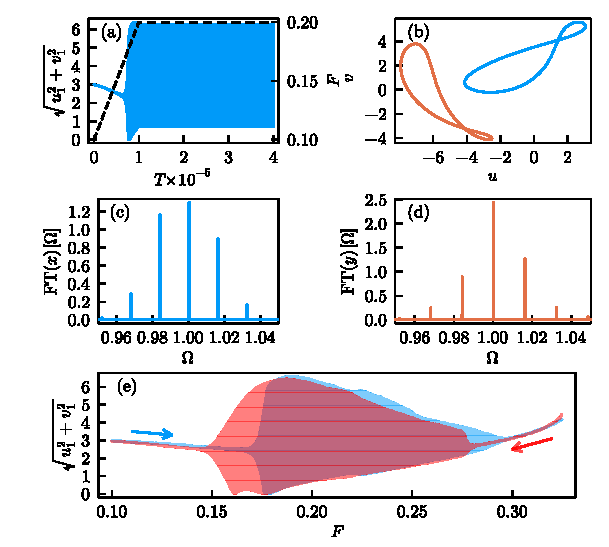
\includegraphics{figures/limit_cycles/2_duffings_timedep.pdf}
	\caption{Adiabatic sweeps of the drive strength $F$. (a) A forward sweep followed by free time-evolution. The response of the first resonator, $x(t)$, (blue) and the value of $F$ (black, dashed) as a function of time. The low-amplitude steady-state branch is followed until $T = 0.8\cross10^{5}$, where limit cycle behaviour sets in. (b) The corresponding phase space paths of (blue) $u_1, v_1$ and (orange) $u_2, v_2$ after the disappearance of transient behaviour. (c,d) The Fourier components of $x(t)$ and $y(t)$. (e) Forward (blue) and backward (red) sweeps over a larger $F$ range, both starting and finishing in stable regions of the low-amplitude branch. In (e), a small additive noise term was added to the harmonic equations to ensure a fast decay of unstable solutions. Parameters used: same as in Fig.~\ref{fig:hopf_ansatz0}.}
	\label{fig:hopf_timedep}
\end{figure}

%While limit-cycle behaviour appears in both sweep directions, it does not cover the entire $F_0$ range.
 
\subsubsection{Gauge-fixed extended harmonic ansatz}

We now proceed to characterise limit cycles by proposing a pair of emergent harmonics equally spaced around $\omega$. This necessitates $11+1$ variables -- 11 harmonic ones ($u, v$), and the limit cycle frequency $\omega_{\rm lc}$,
\begin{multline*}
x(t) = u_1 \cos(\omega t) + v_1 \sin(\omega t) \\
 + u_3 \cos[(\omega + \omega_{\rm lc}) t] + v_3 \sin[(\omega + \omega_{\rm lc}) t] + u_4 \cos[(\omega - \omega_{\rm lc}) t] + v_4 \sin[(\omega - \omega_{\rm lc}) t]
\end{multline*}
\vspace*{-1em}
\begin{multline} \label{eq:hopf_egfa}
y(t) = u_2 \cos(\omega t) + v_2 \sin(\omega t) \,, \\
 + u_5 \cos[(\omega + \omega_{\rm lc}) t] + v_5 \sin[(\omega + \omega_{\rm lc}) t] + u_6 \cos[(\omega - \omega_{\rm lc}) t] \,,
\end{multline}
which results in 12 harmonic equations, see Appendix~\ref{app:harmeqs_2duff_lc}. Due to gauge fixing, the ansatz \eqref{eq:hopf_egfa} does not include a variable $v_6$. The B\'{e}zout bound on the number of steady states is $3^{12} = 531441$. Finding these is still feasible on a single-core computer using homotopy continuation. Despite the high upper bound, the number of real solution branches observed is 10. Out of these, 6 are discarded for having $\omega_{\rm lc} = 0$. Taking into account the inherent fourfold degeneracy [see the discussion of Eq.~\eqref{sec:hopf_hb}], we are left with a single solution branch, as shown in Fig.~\ref{fig:hopf_lc_ss}. The extended ansatz correctly predicts limit cycle behaviour in the region where the single-harmonic ansatz showed Hopf instabilities. Remarkably, both the amplitudes and $\omega_{\rm lc}$ of the limit cycles agree with time-dependent simulation results.

\begin{figure} [h!]
	\centering
	\includesvg[]{figures/limit_cycles/lc_ansatz.svg}
	\caption{(a), (b) Steady states of the coupled Duffing oscillators found using the extended gauge-fixed ansatz \eqref{eq:hopf_egfa} (opaque) overlaid on those found with the single-harmonic ansatz \eqref{eq:hopf_ansatz0} (grey, faded). Stable (full) and unstable (dotted) solutions are shown. Points mark corresponding time-dependent simulation results. (c),(d) The amplitudes corresponding to the two emergent limit cycle harmonics for (red) $x(t)$ and (purple) $y(t)$. (e) The limit cycle frequency.  Parameters used: same as in Fig.~\ref{fig:hopf_ansatz0}.}
	\label{fig:hopf_lc_ss}
\end{figure}

The small inaccuracies of the extended ansatz likely stem from its incompleteness. Fig.~\ref{fig:hopf_timedep}(c),(d) shows that multiple equally-spaced peaks appear in the full response, prompting the need for more harmonics in the ansatz. 
However, adding a further harmonic pair, $\omega \pm 2 \omega_{\rm lc}$, would result in a 20-variable system with up to $3^{20}$ solutions, which is currently outside of our computational capabilities to solve. 


\section{Geometric phases in harmonic systems}

It is instructive to view our $U(1)$ gauge freedom from the perspective of \textit{geometric} or \textit{Berry} phases. These are observed in systems featuring a phase freedom, where an adiabatic variation of the system parameters may induce a change of the free phase~\cite{Cohen_2019, Berry_1988}. While most canonical examples use the phase freedom of a quantum-mechanical wavefunction, geometric phases in classical systems~\cite{Hannay_1985} and their relation to Hopf bifurcations~\cite{Ning_1992a, Ning_1992b} are also known. Here, we briefly note how to describe the phenomenon within the harmonic balance framework. We return to the complex form \eqref{eq:hopf_ansatz_gen} of our harmonic ansatz, absorbing all phases of the solution in a matrix $\tilde{\phi}(T)$, 
\begin{equation}
x(t) = e^{i \tilde{\phi}(T)} \vb{a} + \text{c.c.} \,.
\end{equation}
with $\vb{a}$ containing the harmonic variables, see Eq.~\eqref{eq:hopf_a}.
The time evolution of $\tilde{\phi}(T)$ stems from the underlying harmonics which we denoted by the matrix $\tilde{\omega}$. In addition, we will assume an adiabatic variation of some system parameter $\lambda$, so that
\begin{equation}
\der{\tilde{\phi}(T)}{T} = \tilde{\omega} + T \der{\tilde{\omega}}{T} = \tilde{\omega} + T \frac{\partial \omega}{\partial \lambda} \der{\lambda}{T}\,.
\end{equation}
After following a closed path in parameter space from $\lambda_0$ at time $T_0$ to $\lambda_1$ at time $T_1$ such that $\vb{a}_{\lambda_0} = \vb{a}_{\lambda_1}$, we accumulate a phase change
\begin{equation} \label{eq:hopf_geophase}
\delta \tilde{\phi} = \tilde{\omega} \left(T_1-T_0 \right) +  \int T \frac{\partial \tilde{\omega}}{\partial \lambda} \, d\lambda(T)\,.
\end{equation}
The first term on the right hand side in Eq.~\eqref{eq:hopf_geophase} is the \textit{dynamic phase} -- the phase accumulated solely due to free time-evolution. The second term corresponds to the \textit{geometric phase}, $\delta \tilde{\phi}_g$.

In systems with intact DTTS, as well as in systems featuring subharmonics (see Sec.~\ref{sec:hopf_discrete}), the terms contained in $\tilde{\omega}$ are fixed by an external drive frequency. Varying its phase then induces a geometric phase. For example, in the driven Duffing oscillator example shown in Sec.~\ref{sec:hopf_discrete}, we had $\tilde{\omega} = \text{diag} \{\omega/5 \,, 3\omega/5 \,, \omega\}$. Upon advancing the drive phase $\psi$ by $2\pi$, we have,
\begin{equation}
\delta \tilde{\phi}_g = \int_0^{2\pi} T \frac{\partial \tilde{\omega}}{\partial \psi} \, d\psi(T) =  \frac{\partial \tilde{\omega}}{\partial \omega} \int_0^{2\pi} d\psi(T) = 2\pi\, \text{diag}\{1/5 ,\, 3/5, \, 1\}\,,
\end{equation}
The system has thus transitioned from one of the five degenerate states into another. %If a different parameter than $\omega$ is varied, no phase change occurs. 

In systems featuring limit cycles, evaluating $\partial{\omega} / \partial \lambda$ is less straightforward, since all system parameters, including $\omega$, may affect the limit cycle frequency $\omega_{\rm lc}$. Applying the same protocol to the coupled Duffing oscillators with an extended harmonic ansatz [see Eq.~\eqref{eq:hopf_2duff}], we have
\begin{equation}
\tilde{\omega} = \left \{ \omega ,\, \omega ,\, \omega + \omega_{\rm lc} ,\,  \omega + \omega_{\rm lc} ,\,  \omega - \omega_{\rm lc} , \,  \omega - \omega_{\rm lc} \right\} \,,
\end{equation}
which gives
\begin{equation} \label{eq:hopf_geoshift}
\delta \tilde{\phi}_g = 2 \pi \frac{\partial \tilde{\omega}}{\partial \omega} = 2\pi \left[\mathbb{1} + \frac{\partial \omega_{\rm lc}}{\partial \omega } \text{diag}(0,0,1,1,-1,-1) \right]  \,.
\end{equation}
The first term in the brackets is inconsequential, while the second term only affects the limit cycle variables. The effect of $\delta \tilde{\phi}_g$ is then equivalent to transforming $\vb{a}$ within the degenerate solution manifold\footnote{Note that even though our geometric phase takes the form of a matrix, the phase shift operations are still isomorphic to the $U(1)$ group. As such, they are commutative and do not enable non-Abelian braiding.}. The induced geometric phase is then permanently stored in the limit cycle. Intuitively, the adiabatic change of $\psi$ can be seen as a temporary shift of the drive frequency $\omega$, which "speeds up" (or "slows down") the limit cycle for a limited amount of time, before returning to the original value, leaving a phase change behind it.

\begin{figure} [h!]
	\centering
	\includesvg{figures/limit_cycles/geophase.svg}
	\caption{(a) The dependence of the limit cycle frequency $\omega_{\rm lc}$ on the drive frequency $\omega$ obtained using (line) the gauge-fixed ansatz \eqref{eq:hopf_egfa} and (points) time-dependent simulations. The gradient at $\omega=1.03$ is -0.35 and -0.26, respectively. (b) The evolution of the geometric phase $\delta \phi_g$ during a sweep of the drive phase $\psi$ with $\omega=1.03$. Obtained from a full time-dependent simulation of the sweep, subsequent Fourier transformation and phase extraction of the $\omega - \omega_{\rm lc}$ peak. Numerical data (points) and a linear fit (line), showing a gradient -0.27.}
	\label{fig:hopf_lc_phase}
\end{figure}

We demonstrate the geometric phase concept in Fig.~\ref{fig:hopf_lc_phase}. Using the system parameters from Example \ref{sec:hopf_example}, we compute $ \omega_{\rm lc}$ as a function of $\omega$ [Fig.~\ref{fig:hopf_lc_phase}(a)] and extract the gradient $\partial \omega_{\rm lc} / \partial \omega$. In Fig.~\ref{fig:hopf_lc_phase}(b), we show the accumulated geometric phase $\delta \phi_g$ when sweeping the drive phase $\psi$. The gradients obtained from fully numerical time-evolution agree quite closely, validating Eq.~\eqref{eq:hopf_geoshift}. The gauge-fixed ansatz \eqref{eq:hopf_egfa} yields a slightly different result, but agrees qualitatively. As before, using a larger ansatz may improve the accuracy, but is outwith our computational possibilities. 

\subsubsection{Application: Kerr solitons}

The phase shift in limit cycles we have introduced above may seem like a rather abstract effect. An interesting area of application arises in nonlinear optical ring-cavities. The electric field in a ring cavity is described by a set of spatial modes with equally-spaced wavenumbers. In the presence of a Kerr nonlinearity and a periodic drive, responses can be observed where many of these modes oscillate at equally-spaced frequencies, forming a frequency comb. In real space, such a response appears as a highly-localised field profile circulating in the ring cavity -- a so-called \textit{Kerr soliton}~\cite{Weng_2022, Lugiato_2018, Herr_2012}. Because of this feature, Kerr solitons are a promising avenue for realising pulsed lasers. 

We may view the soliton behaviour as a limit cycle. We describe it with a harmonic ansatz similar to Eq.~\eqref{eq:hopf_extansatz}, such that the electric field in the ring cavity reads
\begin{equation}
E(\theta, t) = \sum_{k = -K}^{K} a_k \e^{i \left[\left(\omega + k \omega_{\rm lc} \right)t - k \theta \right]} \,,
\end{equation}
where $\theta \in [0, 2\pi)$ is the cavity's angular coordinate. By tuning the drive phase $\delta \psi$, we may again apply a geometric phase $\delta \phi_g$, shifting each $a_k$ proportionally to $k$ [cf.~Eq.~\eqref{eq:hopf_geoshift}], 
\begin{equation}
a_k \rightarrow a_k \e^{i k \delta{\phi}_g} \,, \qquad \delta \phi_g = \frac{\partial \omega_{\rm lc}}{\partial \omega} \delta \psi \,,
\end{equation}
which is equivalent to changing the angular position $\theta$ by $\delta \theta = -\delta \phi_g$. By tuning the drive phase, we may therefore achieve precise control of the soliton's position. 

This mechanism is currently being explored as a means to synchronize Kerr solitons~\cite{Jang_2015, Erkintalo_2022}. The necessary gradient of limit cycle frequency against drive frequency has been measured experimentally in a different context~\cite{Bao_2017}. The analysis in this Section provides a general explanation of the phenomenon, complementary to the prevalent system-specific descriptions such as the Lugiato-Lefever equation~\cite{Lugiato_1987}. 